\chapter{Study 1: diagrams of themes}\label{ch:S1_Diagrams}
The results of Study 1 were analysed using an inductive approach of thematic analysis: there was no pre-existing coding scheme. From this analysis, 51 codes were established, which were grouped into eight themes. Each theme was visualised in a diagram, which shows the theme's main codes and relationships between codes, as well as quotes in dotted squares to exemplify what type of quotes were grouped under this code. The numbers in parentheses indicate the number of quotes, and the number of interviewees who mentioned it. 
The description of each theme is accompanied with notes and quotes taken from the transcripts to further illustrate when this theme was mentioned. These serve as examples and are not all the instances of a theme. To differentiate notes from verbatim quotes, the quotes are in italics and double quotation marks. Words put in brackets are added by the researcher to make the quote more understandable for the reader, for instance if the interviewee is talking about 'it' or 'them'. The diagrams are ordered according to the number of quotations associated with a theme, with the theme with the most quotations listed first. The only exception is the 'Other' theme which is described last.

\newpage

\section{Task}
Quotes were grouped under this theme if participants described things that were particular to their task, for instance how they structured their task, whether they switched tasks, and how long they took to complete tasks.

\begin{figure}[!ht]
\centering
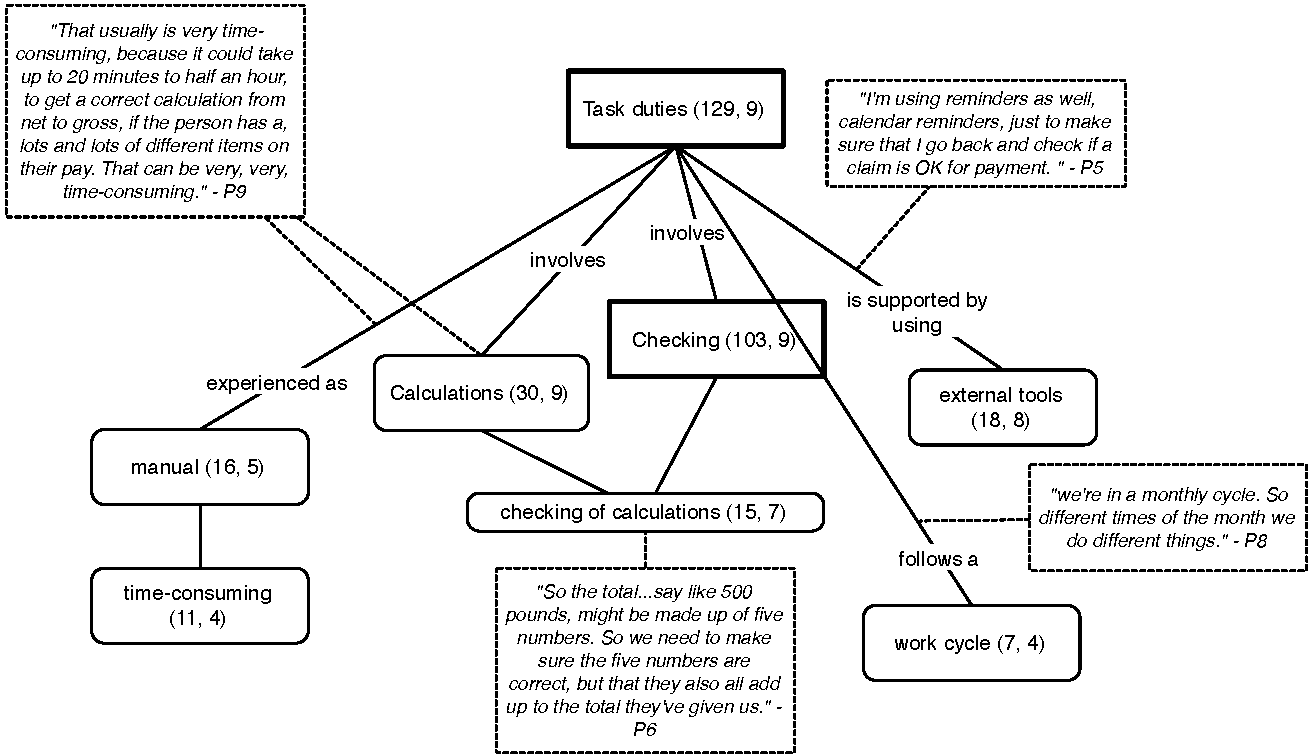
\includegraphics[width=\textwidth]{images/ch12/Task.pdf}
\caption[Study 1 Task diagram]{Diagram showing the theme Task. The numbers in parentheses indicate the number of quotes and the number of participants who mentioned it, respectively.}
\vspace{-9pt}
\label{fig:ch3_task}
\end{figure}

\section{Checking}\label{subsec:Checking}
Quotes were grouped under this theme if participants talked about checking data input as part of their job. 

\begin{figure}[!ht]
\centering
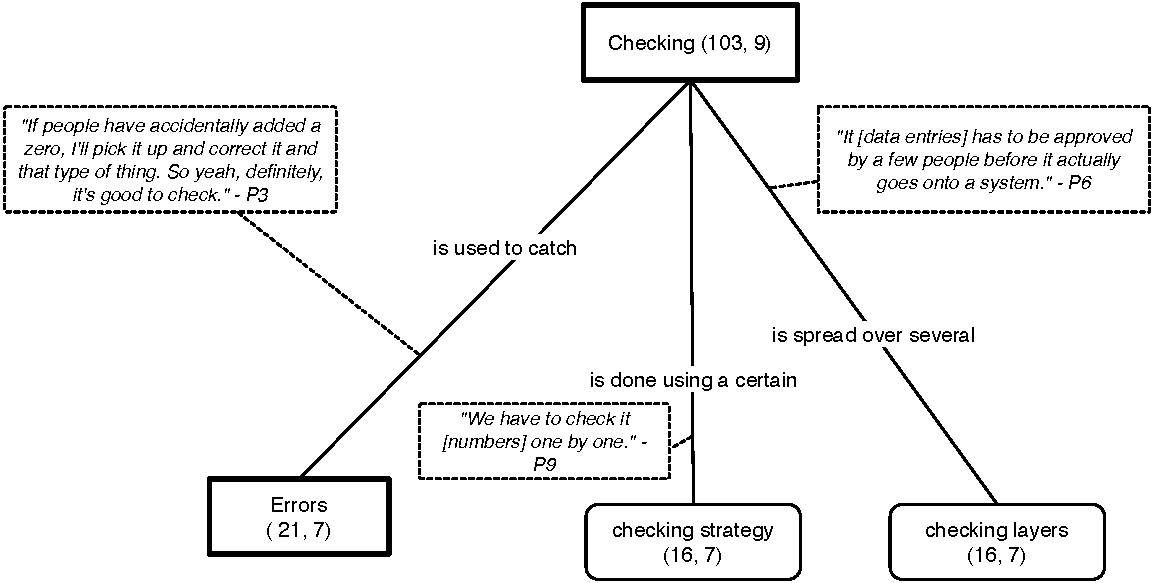
\includegraphics[width=\textwidth]{images/ch12/Checking.pdf}
\caption[Study 1 Checking diagram]{Diagram showing the theme Checking.}
\vspace{-9pt}
\label{fig:ch3_checking}
\end{figure}

\newpage

\begin{table}[htp]
\centering
    \begin{tabular}{ | l | p{10cm} |}
    \hline
     \textbf{Participant} & \textbf{Quote} \\ \hline
    P3 & \textit{"we try and pick it [errors] up and then obviously there's all the different stages that pick it up as you go along."}\\ \hline
    P9 & \textit{"the departments actually sometimes treat us as a checking system [laughs], but they shouldn't really, the schools. Because we're here just to make sure that people get paid correctly. But even though we are like a second check, we feel sometimes that we are the first checkpoint."} \\ \hline
    P7 & \textit{"All this piece of work, when we input in the system, will be actually checked by another person... my manager will print it out, and then check... other colleagues will double-check it for you as well, the calculations."} \\ \hline
    P8 & \textit{"one of these errors could be things that are missed during the checking."} \\ \hline

    \hline
    \end{tabular}
    \caption[Study 1 checking quotes]{Verbatim quotes taken from the interview transcripts that were about checking.}
    \label{table:ch3_checkingquotes}
\end{table}%

\begin{table}[htp]
\centering
    \begin{tabular}{ | l | p{10cm} |}
    \hline
     \textbf{Participant} & \textbf{Quote/note} \\ \hline
    P1 &  first puts in all the details, then when done checks everything against the source. \\ \hline
    P7 & when entering numbers from paper to computer, mostly looked at paper form and the number pad; only looked at screen after finishing entering all the numbers from the form to check. \\ \hline
    P5 & \textit{"We would go by the receipt, so we would try to make sure that the receipts are in order."} \\ \hline

    \hline
    \end{tabular}
    \caption[Study 1 checking own input]{Checking own input when entering data.}
    \label{table:ch3_owninputquotes}
\end{table}%

\begin{table}[htp]
\centering
    \begin{tabular}{ | l | p{10cm} |}
    \hline
     \textbf{Participant} & \textbf{Quote} \\ \hline
    P5 &  \textit{"The numbers on the expense form will be checked individually. So the total will obviously be, say like 500 pounds, might be made up of five numbers. So we need to make sure the five numbers are correct, but that they also all add up to the total they've given us."} \\ \hline
    P6 & \textit{"The numbers on the expense form will be checked individually."}\\ \hline
    P9 & \textit{"We have to check it one by one."} \\ \hline

    \hline
    \end{tabular}
    \caption[Study 1 checking other people's input]{Checking other people's input.}
    \label{table:ch3_otherinputquotes}
\end{table}%

\newpage

\section{System}
Quotes were grouped under this theme if participants talked about the computer system they were using to input data. 

\begin{figure}[!ht]
\centering
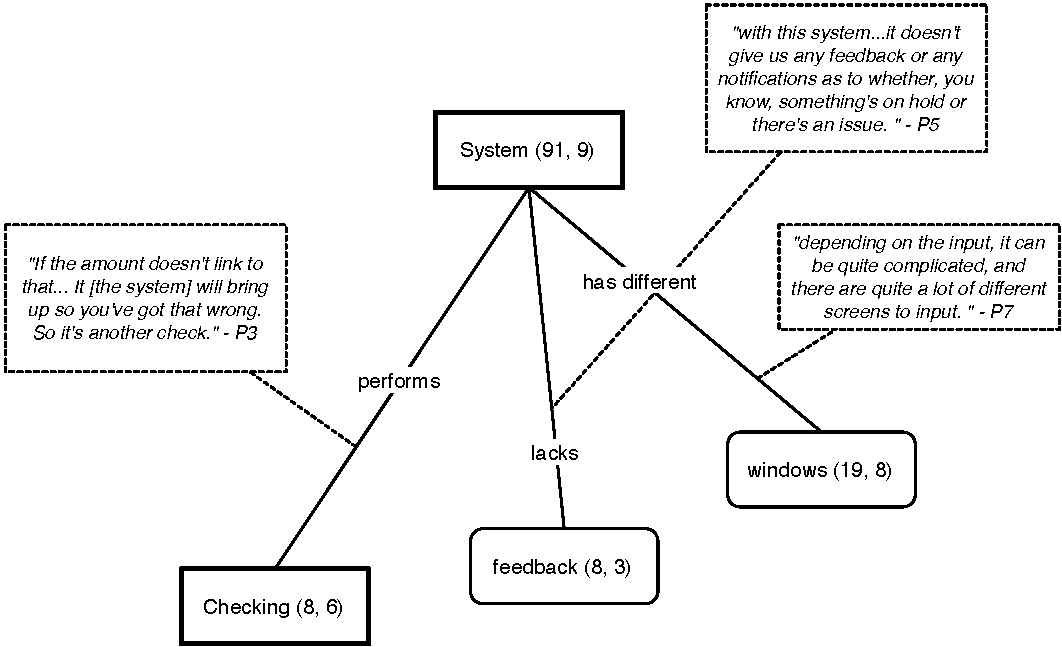
\includegraphics[width=\textwidth]{images/ch12/System.pdf}
\caption[Study 1 System diagram]{Diagram showing the theme System.}
\vspace{-9pt}
\label{fig:ch3_system}
\end{figure}

\section{Environment}
Quotes were grouped under this theme if participants described their environment, for instance if they talked about their physical work setting, and the work culture of their organisation. 

\begin{figure}[!ht]
\centering
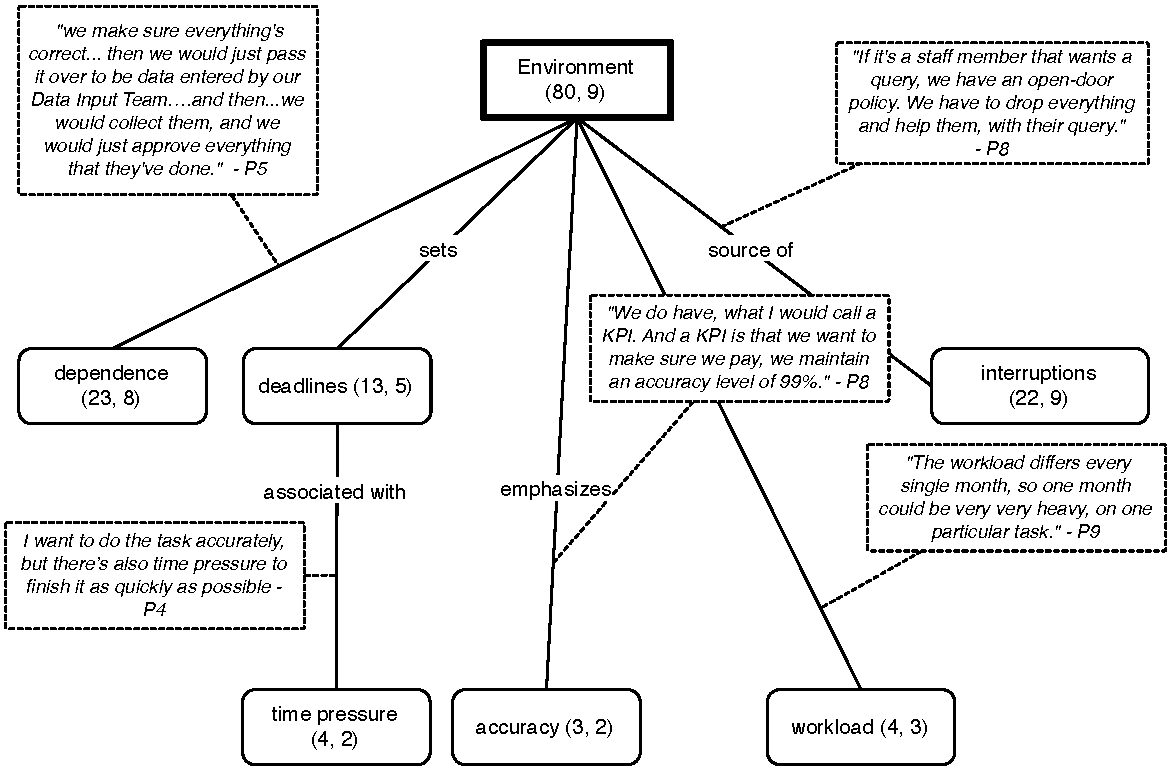
\includegraphics[width=\textwidth]{images/ch12/Environment.pdf}
\caption[Study 1 Environment diagram]{Diagram showing the theme Environment.}
\vspace{-9pt}
\label{fig:ch3_environment}
\end{figure}

\newpage

\section{Data}
Quotes were grouped under this theme if participants described the data they were dealing with, for instance the type and length of data items, and from which source they copied data.

\begin{figure}[!ht]
\centering
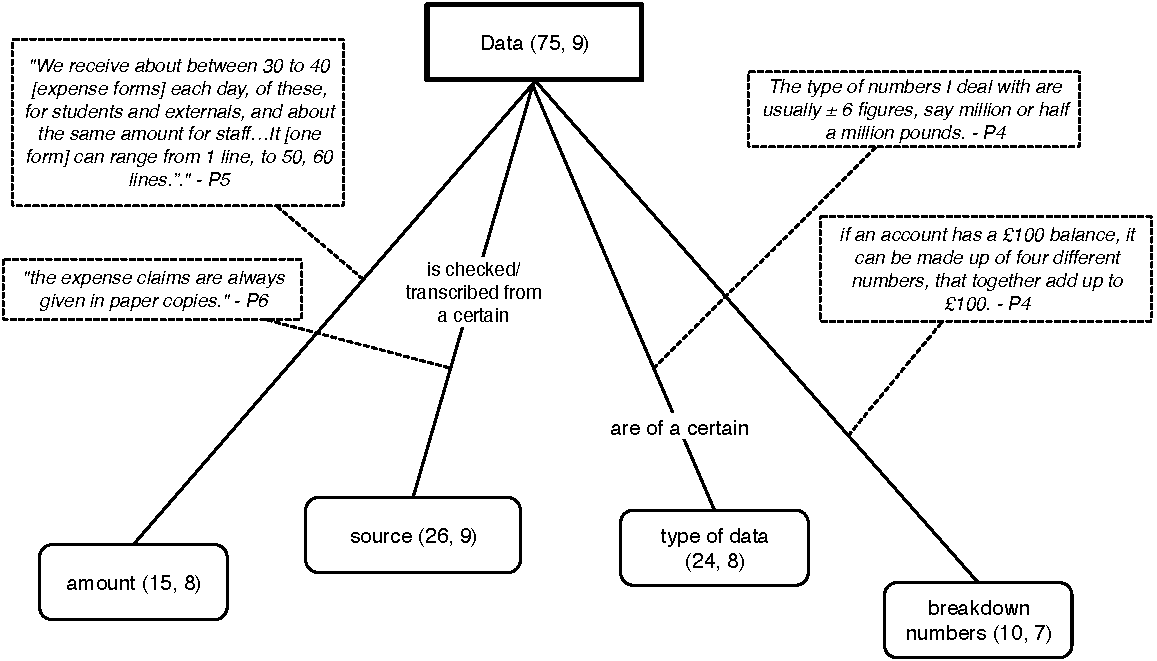
\includegraphics[width=\textwidth]{images/ch12/Data.pdf}
\caption[Study 1 Data diagram]{Diagram showing the theme Data.}
\vspace{-9pt}
\label{fig:ch3_data}
\end{figure}

\section{Errors}
Quotes were grouped under this theme if participants described situations where errors were made: who made them, why were they made, what were the consequences. 

\begin{figure}[!ht]
\centering
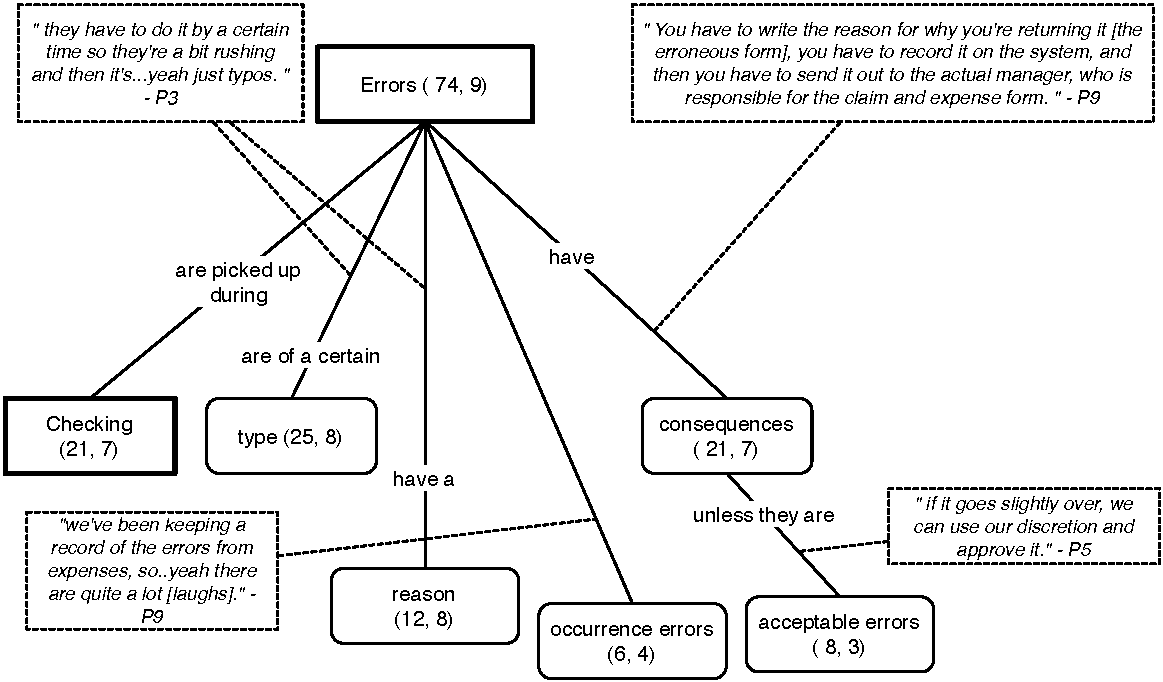
\includegraphics[width=\textwidth]{images/ch12/Errors.pdf}
\caption[Study 1 Errors diagram]{Diagram showing the theme Errors.}
\vspace{-9pt}
\label{fig:ch3_errors}
\end{figure}

\newpage

\begin{table}[htp]
\centering
    \begin{tabular}{ | l | p{10cm} |}
    \hline
     \textbf{Participant} & \textbf{Quote/note} \\ \hline
    P6 &  \textit{"it's quite common that we have to return an expense or payment back to someone. It happens quite often, yeah."} \\ \hline
    P4 & Yes all the time, lots of typos.\\ 
    \hline
    \end{tabular}
    \caption[Study 1 errors quotes]{People mentioned errors occur quite frequently.}
    \label{table:ch3_occurrenceerrorsquotes}
\end{table}%


\begin{table}[htp]
\centering
    \begin{tabular}{ | l | p{10cm} |}
    \hline
     \textbf{Participant} & \textbf{Quote} \\ \hline
    P3 &  \textit{"sometimes it's because people have done typos, done too many zeroes, or left out a zero."} \\ \hline
    P5 & \textit{"the expense breakdown doesn't match what (...) whatever they put as the grand total."}\\ 
    \hline
    \end{tabular}
    \caption[Study 1 type of errors quotes]{The type of errors.}
    \label{table:ch3_typeoferrorsquotes}
\end{table}%


\begin{table}[htp]
\centering
    \begin{tabular}{ | l | p{10cm} |}
    \hline
     \textbf{Participant} & \textbf{Quote} \\ \hline
    P9 &  \textit{"Because the departments actually sometimes treat us as a checking system [laughs], but they shouldn't really."} \\ \hline
    P7 & \textit{"Yeah, human laziness or something [laughs]."}\\ \hline
    P8 & \textit{"sometimes, you know, through human error, you know, things don't get paid properly."} \\
    \hline
    \end{tabular}
    \caption[Study 1 reasons for errors quotes]{The reasons for errors.}
    \label{table:ch3_errorreasonsquotes}
\end{table}%


\begin{table}[htp]
\centering
    \begin{tabular}{ | l | p{10cm} |}
    \hline
     \textbf{Participant} & \textbf{Quote/note} \\ \hline
    P5 &  \textit{"generally we tend, we try not to send claims back to departments because they might get lost in the post, and it's an inconvenience as well. So we try to... resolve it ourselves.."} \\ \hline
    P4 & We allow a certain amount of tolerance; if it turns out the thing you bought has actually decreased value and is now  \pounds40, we will allow to return  \pounds50\\ \hline
    P7 & \textit{"we normally e-mail the budget holder to say... what you authorised is actually different. But for this kind of thing, it's only 10 pounds...we normally just process this without contacting them."} \\ \hline

    \hline
    \end{tabular}
    \caption[Study 1 acceptable errors quotes]{Acceptable errors.}
    \label{table:ch3_acceptableerrorsquotes}
\end{table}%

\clearpage
\section{Strategy}
Quotes were grouped under this theme if participants described the strategies they used to carry out their task.  

\begin{figure}[!ht]
\centering
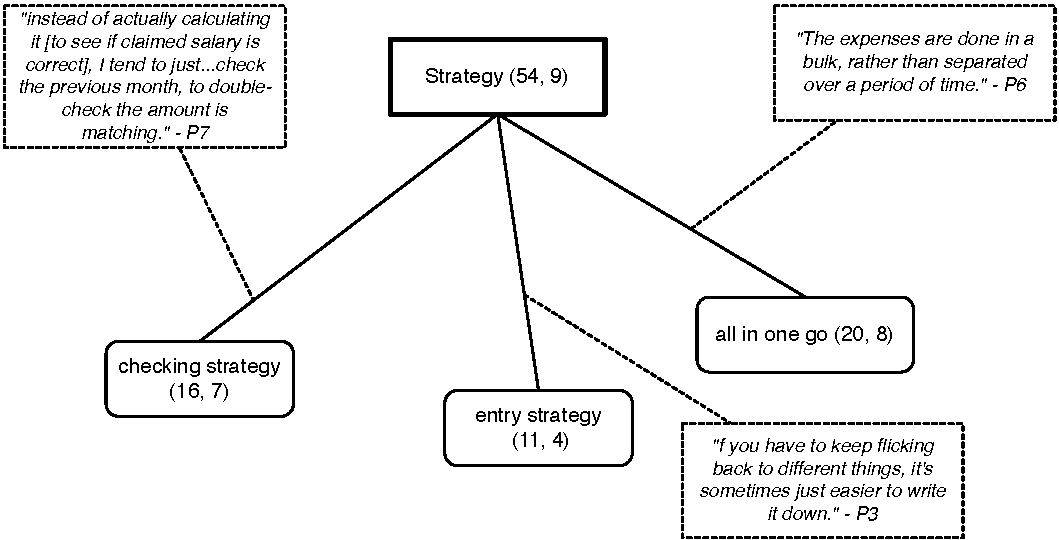
\includegraphics[width=\textwidth]{images/ch12/Strategy.pdf}
\caption[Study 1 Strategy diagram]{Diagram showing the theme Strategy.}
\vspace{-9pt}
\label{fig:ch3_strategy}
\end{figure}

\begin{table}[htp]
\centering
    \begin{tabular}{ | l | p{10cm} |}
    \hline
     \textbf{Participant} & \textbf{Quote/note} \\ \hline
    P3 &  \textit{"I just try and do it in the quickest way...It's nice, once you've done it, it's completed, so it's sort your weight lifted [laughs]. So you don't need to think about it again."} \\ \hline
    P6 & \textit{"the expenses are done in a bulk, rather than separated over a period of time. When I'm doing it lots at a time, I think once you get into sort of the hang of it, it gets done a lot quicker than..you just get used to putting them in, and inputting it all."} \\ \hline
    P9 & \textit{"I try to concentrate on my task...I try to do one task [i.e. doing all expenses], finish one, and then do another."} \\ \hline
    P4 &  It's difficult to take rests or even switch in-between number entry tasks because of the work pressure, and feels pressure by boss. \\ 
    \hline
    \end{tabular}
    \caption[Study 1 batching quotes]{Most participants entered all numbers in one go.}
    \label{table:ch3_inonegoquotes}
\end{table}%

\begin{table}[htp]
\centering
    \begin{tabular}{ | l | p{10cm} |}
    \hline
     \textbf{Participant} & \textbf{Quote/note} \\ \hline
    P3 &  \textit{" I wouldn't necessarily have to [memorise numbers], It's more just if you have to keep flicking back to different things, it's sometimes just easier to write it down, or just try and remember it. But you can obviously take the long version and keep flicking back to the correct screen."} \\ \hline
    P2 & \textit{"we have different grants and different project codes as a result, but you, because you use them so much, you end up remembering them."} \\ \hline
    \end{tabular}
    \caption[Study 1 strategy quotes]{Examples of strategies people used.}
    \label{table:ch3_strategiesquotes}
\end{table}%

\ \clearpage

\section{Importance of accuracy and paper trails}
Quotes were grouped under this theme if participants talked about the sensitivity of financial data, which is why not all people were authorised to approve or access financial data, and the importance of a paper trail for data entries. 

\begin{figure}[!ht]
\centering
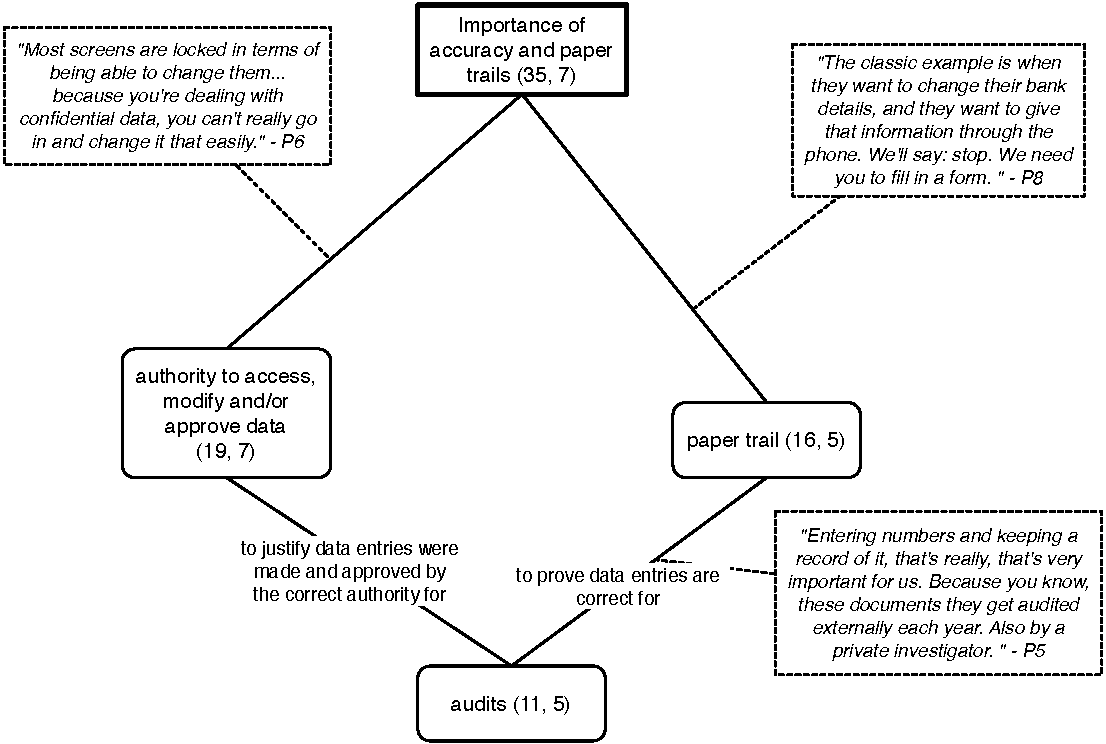
\includegraphics[width=\textwidth]{images/ch12/Papertrail.pdf}
\caption[Study 1 Importance of accuracy and paper trails diagram]{Diagram showing the theme 'Importance of accuracy and paper trails'.}
\vspace{-9pt}
\label{fig:ch3_papertrail}
\end{figure}

\section{Other}
Quotes were grouped under this theme if participants talked about things that did not fit into any other category but were still considered relevant, such as issues participants experienced, or queries they often received.

\begin{figure}[!ht]
\centering
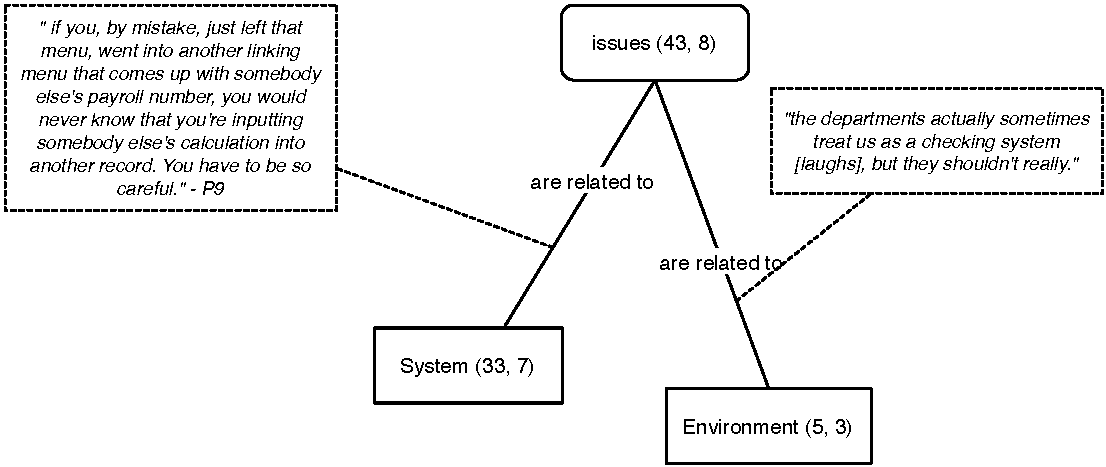
\includegraphics[width=\textwidth]{images/ch12/Other.pdf}
\caption[Study 1 Other diagram]{If people described issues, it usually had to do with the system.}
\vspace{-9pt}
\label{fig:ch3_other}
\end{figure}

\begin{table}[htp]
\centering
    \begin{tabular}{ | l | p{10cm} |}
    \hline
     \textbf{Participant} & \textbf{Quote/note} \\ \hline
    P5 &  \textit{"There are other issues. You could say I think hundreds, I mean not just with the work that we do on expenses, but across [university A], across [university A] Finance, the Finance division...We just have to kind of work our way around the system and you know, adapt to it."} \\ \hline
    P7 & \textit{"It's only the matter of how you get used to the Payroll system. Because companies have different systems, the data inputting can take a while to get used to it."} \\ \hline
    P9 &  \textit{"You know, all systems are a bit funny, I think. But you just gotta get used to it."} \\ \hline
    \end{tabular}
    \caption[Study 1 issues quotes]{Issues that participants experienced with the system.}
    \label{table:ch3_otherquotes}
\end{table}%


\chapter{Information sheet}\label{ch:information_sheet}
The information sheet given to the participants in Study 1 is shown in Figure \ref{fig:informationsheet}. 

\begin{figure}[htp] \centering{
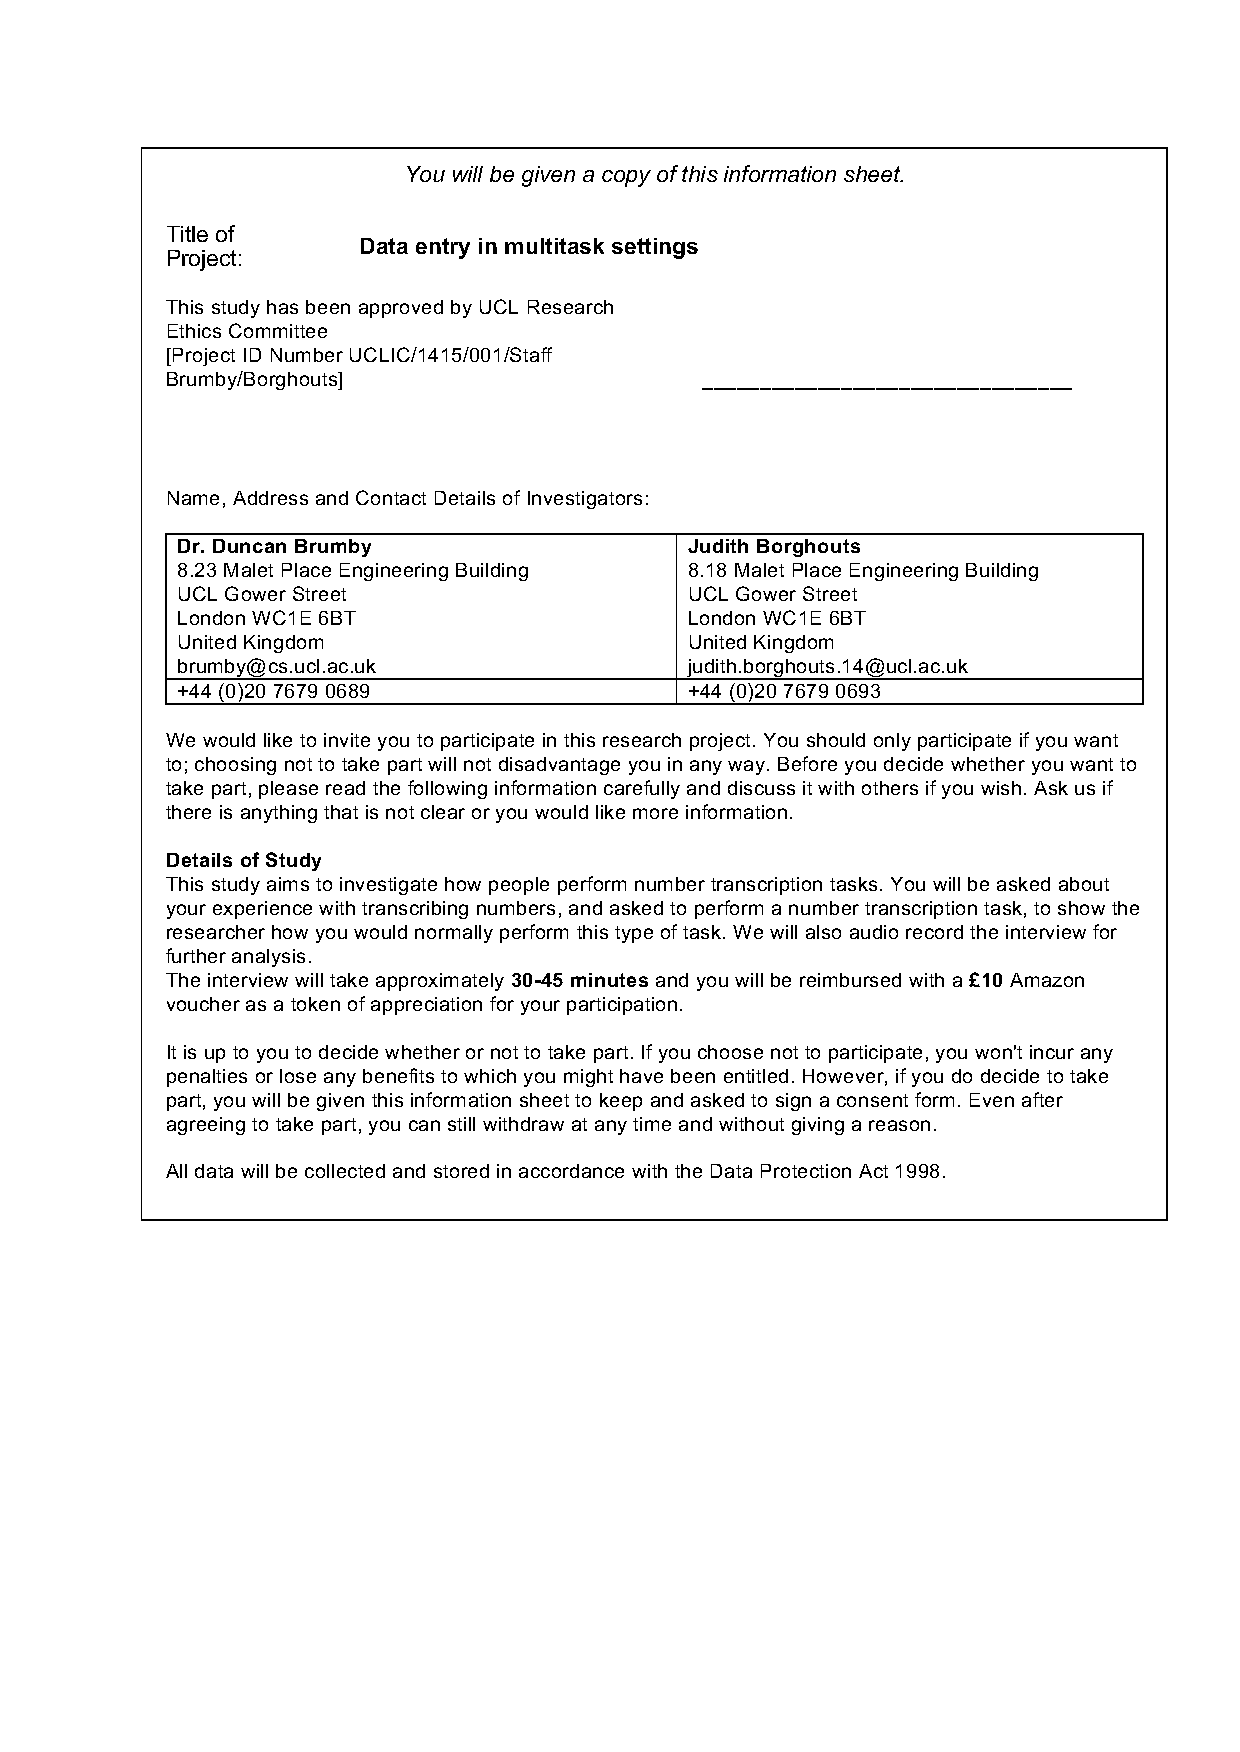
\includegraphics[width=\textwidth,keepaspectratio]{images/Informationsheet.pdf}}
\caption{Information sheet}
\label{fig:informationsheet}
\end{figure} 

\chapter{Consent form}\label{ch:consentform}
The consent form used for Study 1 is shown in Figure \ref{fig:consentform}. 

\begin{figure}[htp] \centering{
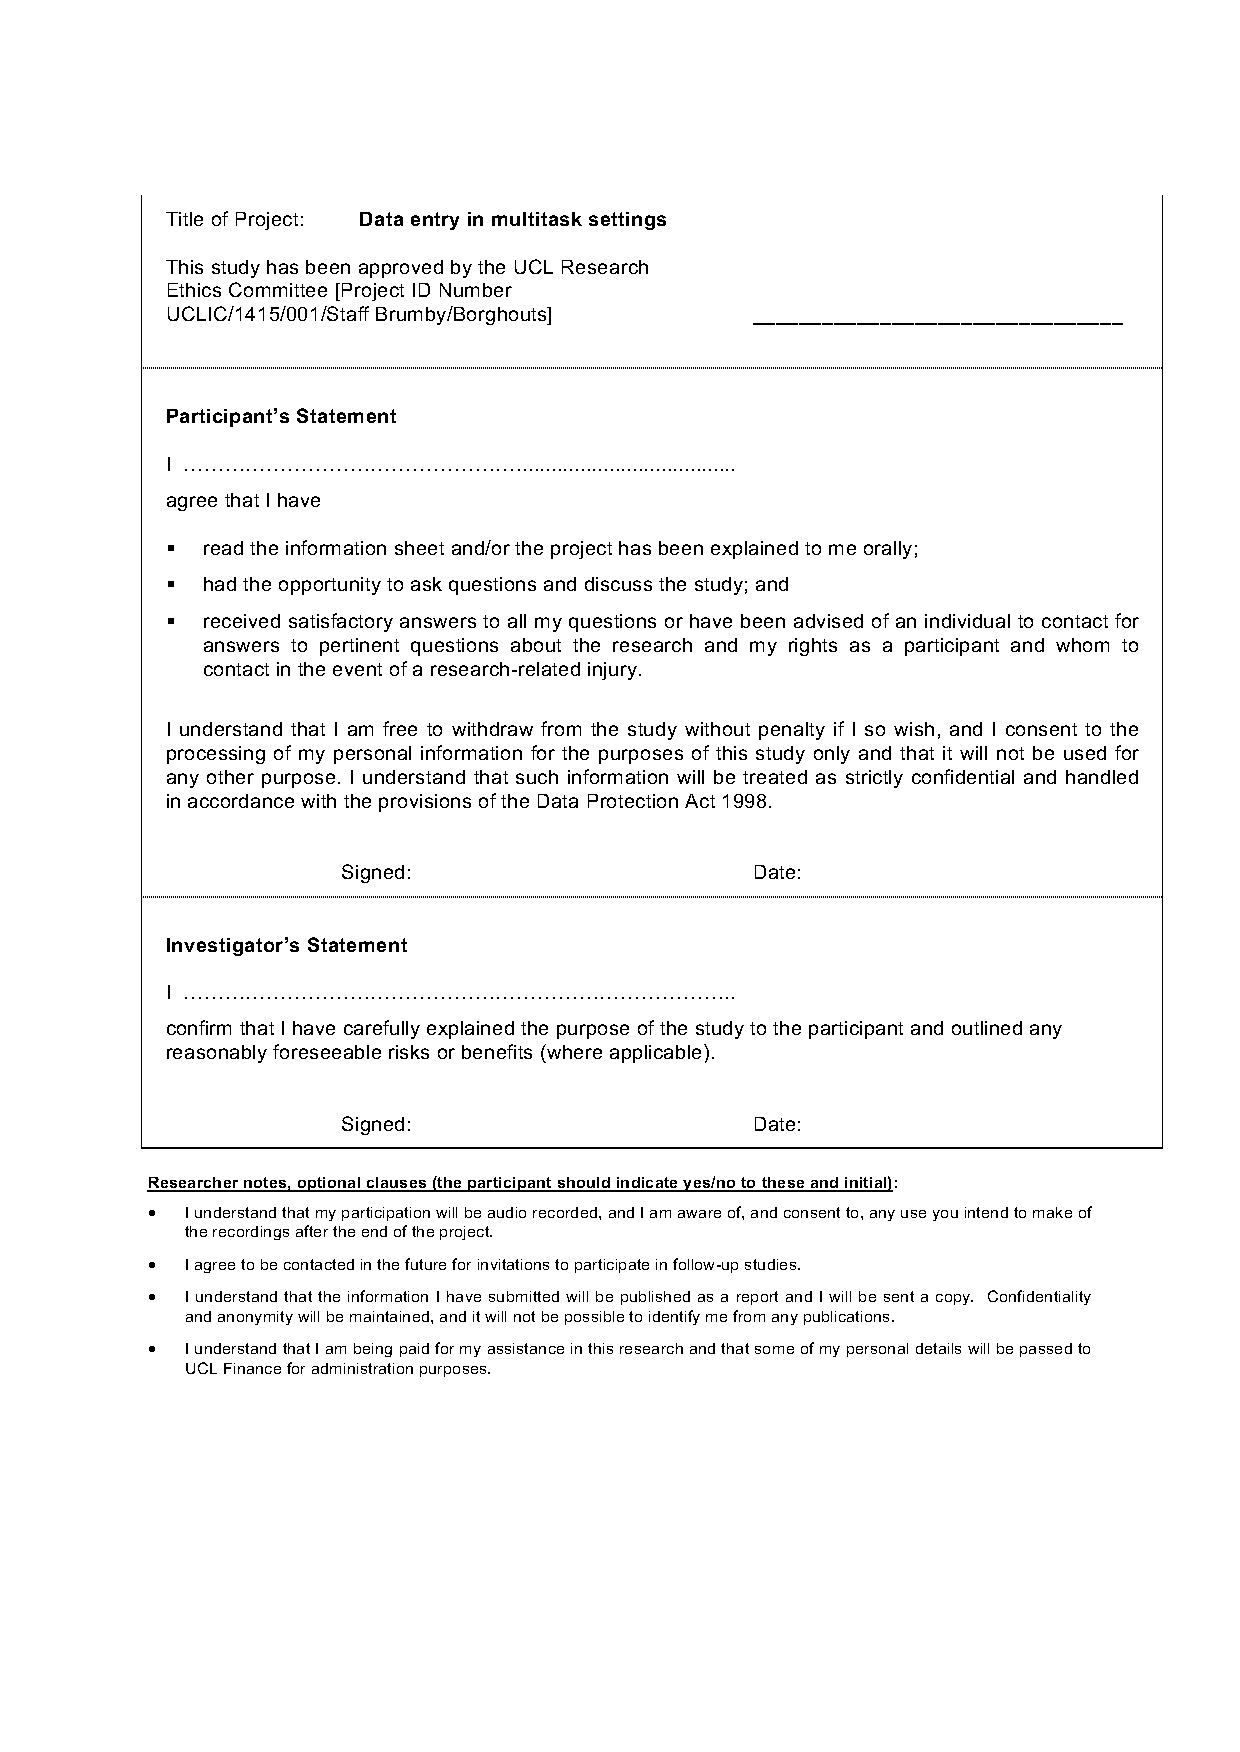
\includegraphics[width=\textwidth,keepaspectratio]{images/Consentform.pdf}}
\caption{Consent form}
\label{fig:consentform}
\end{figure} 

\chapter{Interview script}\label{ch:interviewscript}
The interview script used for Study 1 is given below. This script only served to guide the interview, and does not contain all questions that were asked. Based on what the participant was saying, follow-up questions were asked. 

\subsubsection{Before the interview}
\begin{itemize}
\item 
ensure participant is aware of purpose research 
\item 
explain what will happen
\item 
informed consent
\item 
ask for permission to audio record interview
\end{itemize}
\subsubsection{Work}
\begin{itemize}
\item Tell me something about your work (what do you do)
\item  How many hours per week (full-time/part-time)
\item How long have you been working here (at this company) \item How long have you been doing this type of work
\end{itemize}
\subsubsection{Number entry}
\begin{itemize}
\item  What activities do you do for work that involve transcribing numbers?
e.g. filling in expenses, tax returns, setting up invoices
\item How often do you do this (per day/week)?
\item How many numbers is it roughly that you have to enter?
\item How long do you usually take?
\item What type of numbers? Usually same numbers, or can it be anything?
\item Do you get to enter numbers that are different from your familiar format?
e.g. 2,000 or 2.000; 9/15/14 instead of 15/9/14
\item Do you deal with foreign currencies?
\item Tell me something about how you enter these numbers
\item When do you do these tasks? Immediately when you get them, or save them for later? Morning, afternoon?
\item Does urgency/time pressure influence how you do the task (if so, how)
\item Do you do them in-between other tasks or save a particular part of the day for it?
\item Do you do all tasks all at once, or take rests in between?
(if rests, what do you do? switch to another task, have a coffee, lunch, break, etc.)
\item Do you feel that the way you enter it changes after a while?
e.g. you get better at it so it kind of becomes automatic, or less mentally exhausting? Or is it the opposite, becomes more exhausting?
\item Do you do other things as well during this task
e.g. listening to music, attending to another task
\item Do you sometimes have to briefly store numbers in memory, or calculate them from numbers you already have?
If so, do you use external tools to offload memory?
\item Where do you copy them from? Paper, digital files, combination?
\item Do numbers get checked, to see if they're correct? Do you or anyone else check these numbers?
\item Do you ever get entered numbers from someone else, that you then have to check if they are correct?
\item What is your general experience with transcribing numbers?
e.g. easy, boring, part of the job
\end{itemize}
\subsubsection{Environment}
\begin{itemize}
\item Do you always work in the same environment, or sometimes work in different places, such as at home, or when you're on the train, or working at a cafe? What about number entry tasks?
\item Do you do your work on a desktop, laptop, tablet, anything else? Are some devices harder or easier?
\item How is your desk organized?
\item Do you organise it differently when doing number entry tasks?
\item Do you have notifications on (e.g. e-mail, work-related instant messaging); if you do get new notification, do you attend to it straight away or finish task first?
\item Do you get interrupted in other ways, for example when the phone is ringing, or when a colleague or your boss asks you something? How do you deal with these interruptions? What is your experience with these interruptions?
\item Critical incident: Has there ever been an incident where a mistake in entering a number went undetected, and was discovered later on?
\end{itemize}
\subsubsection{Demonstration}
\begin{itemize}
\item Could you show me the software you use to transcribe numbers?
What is your experience with this system, works well?
(If negative, how do you deal with that? do you use any strategies to make it more optimal for yourself?)
\item Do you feel confident entering the numbers?
\item How do you place your windows?
\item Could you show me how you perform a typical number transcription task (do it how you would normally); if you feel uncomfortable about sharing work data, you can enter any type of numbers, as long as it somewhat resembles data you would normally enter for work
\end{itemize}
\subsubsection{After the interview}
\begin{itemize}
\item Thank participant
\item explain what will happen to their data
\item do they have any more questions
\item clarify when they will be compensated
\item Ask if participant knows any further people who might be suitable and willing to participate
\end{itemize}
